\renewcommand{\thechapter}{A}
\chapter{Appendix}

\begingroup
\footnotesize
\begin{longtable}{>{\RaggedRight\arraybackslash}p{3.5cm} >{\RaggedRight\arraybackslash}p{9.25cm} >{\RaggedRight\arraybackslash}p{2cm}}
    \captionsetup{labelfont=bf, font=footnotesize}
    \caption[Software tools used in this work]{\RaggedRight \footnotesize Software tools used in this work.}
    \label{tab:software}\\
    
    \toprule
\rowcolor{lightgray}
\textbf{Name} & \textbf{Source} & \textbf{Reference} \\ 
\midrule
\endfirsthead

\multicolumn{3}{@{}l}{\RaggedRight \tablename\ \thetable{} -- Continued} \\
\\
\toprule
\rowcolor{lightgray}
\textbf{Name} & \textbf{Source} & \textbf{Reference} \\ 
\midrule \\
\endhead \\
\midrule 
\multicolumn{3}{r}{\footnotesize Continued on next page} \\
\endfoot

\bottomrule
\endlastfoot

\\
Visual Studio Code v1.93.1   & \url{https://github.com/microsoft/vscode}          & --                                    \\
\\
Snakemake v8.29.6            & \url{https://github.com/snakemake/snakemake}       & \cite{koster_snakemakescalable_2012}  \\
\\
Miniforge v24.7.1            & \url{https://github.com/conda-forge/miniforge}     & --                                    \\
\\
VISOR v1.1.2.1               & \url{https://github.com/davidebolo1993/VISOR}      & \cite{bolognini_visor_2020}           \\
\\
minimap2 v2.28               & \url{https://github.com/lh3/minimap2}              & \cite{li_minimap2_2018}               \\          
\\
SAMtools v1.21               & \url{https://github.com/samtools/samtools}         & \cite{danecek_twelve_2021}            \\
\\
SAVANA v1.2.2                & \url{https://github.com/cortes-ciriano-lab/savana} & \cite{elrick_savana_2024}             \\
\\
Severus v1.2                 & \url{https://github.com/KolmogorovLab/Severus}     & \cite{keskus_severus_2024}            \\
\\
Sniffles2 v2.4               & \url{https://github.com/fritzsedlazeck/Sniffles}   & \cite{smolka_detection_2024}          \\
\\
SVision-Pro v2.0             & \url{https://github.com/sonGBowang125/SVision-pro} & \cite{wang_novo_2024}                 \\
\\
BEDtools v2.31.1             & \url{https://github.com/arq5x/bedtools2}           & \cite{quinlan_bedtools_2010}          \\
\\
GW v1.1.1                    & \url{https://github.com/kcleal/gw   }              & \cite{cleal_gw_2024}                  \\
\\
UCSC Genome Browser v2024    & \url{https://genome.ucsc.edu/index.html}           & \cite{perez_ucsc_2025}                \\
\\
Rstudio v2024.04.2           & \url{https://github.com/rstudio/rstudio}           & --                                    \\      
\\

\end{longtable}
\endgroup


\begingroup
\vspace{0.35cm}
\footnotesize
\begin{longtable}{>{\RaggedRight\arraybackslash}p{3.5cm} >{\RaggedRight\arraybackslash}p{2cm} >{\RaggedRight\arraybackslash}p{2cm} >{\RaggedRight\arraybackslash}p{2cm}}
    \captionsetup{labelfont=bf, font=footnotesize}
    \caption[File sizes by coverage]{\RaggedRight \footnotesize Size in gigabytes 
    of long-read sequencing files generated using VISOR toolkit at different 
    sequencing depths. The files include BAM, their indexes (BAI), and 
    unaligned reads in FASTQ files.}
    \label{tab:file_sizes}\\
    
    \toprule
    \rowcolor{lightgray}
    \textbf{Coverage} & \textbf{BAM} & \textbf{BAI} & \textbf{FASTQ} \\ 
    \midrule
    \endfirsthead
    
    \multicolumn{4}{@{}l}{\RaggedRight \tablename\ \thetable{} -- Continued} \\
    \\
    \toprule
    \rowcolor{lightgray}
    \textbf{Coverage} & \textbf{BAM} & \textbf{BAI} & \textbf{FASTQ} \\ 
    \midrule
    \endhead
    
    \midrule 
    \multicolumn{4}{r}{\footnotesize Continued on next page} \\
    \endfoot
    
    \bottomrule
    \endlastfoot
    
    30x\_normal & 112.42 & 0.0347 & 173.17 \\
    30x & 113.20 & 0.0351 & 174.02 \\
    30x & 113.19 & 0.0350 & 174.02 \\
    30x & 113.22 & 0.0350 & 174.02 \\
    50x\_normal & 187.01 & 0.0551 & 288.58 \\
    50x & 188.71 & 0.0556 & 289.99 \\
    50x & 188.85 & 0.0556 & 289.99 \\
    50x & 188.70 & 0.0556 & 289.99 \\
    100x\_normal & 374.24 & 0.1060 & 577.11 \\
    100x & 377.85 & 0.1071 & 579.93 \\
    100x & 377.86 & 0.1071 & 579.92 \\
    100x & 377.72 & 0.1071 & 579.93 \\
    200x\_normal & 748.34 & 0.2079 & 1157.12 \\
    200x & 754.99 & 0.2099 & 1157.12 \\
    200x & 754.89 & 0.2099 & 1157.12 \\
    200x & 755.35 & 0.2099 & 1157.12 \\
    \midrule
    \textbf{Total} & 5726.54 & 1.6266 & 8219.22 \\

\end{longtable}
\endgroup


\begin{figure}[H]
    \centering
    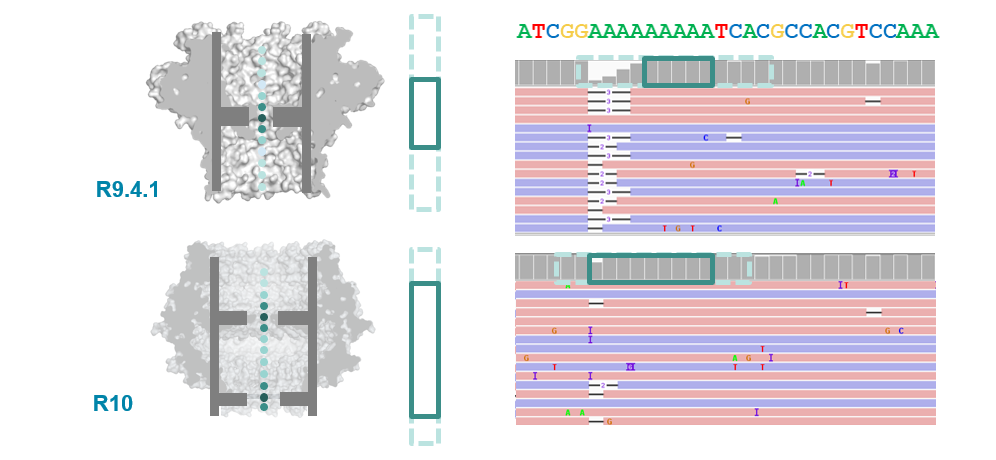
\includegraphics[width=\textwidth]{img/ont_pores.png}
    \caption[R10 nanopore improvements over R9]{The R10 nanopore design introduces 
    key improvements over its R9 predecessor: a longer barrel and dual reader head 
    architecture. These structural enhancements enable improved resolution of 
    homopolymeric regions such as VNRTs, significantly increasing the consensus 
    accuracy of nanopore sequencing data. Reproduced from 
    \cite{oxford_nanopore_technologies_r103_2020}.}
    \label{fig:ont_pores}
\end{figure}


\begin{figure}[H]
    \centering
    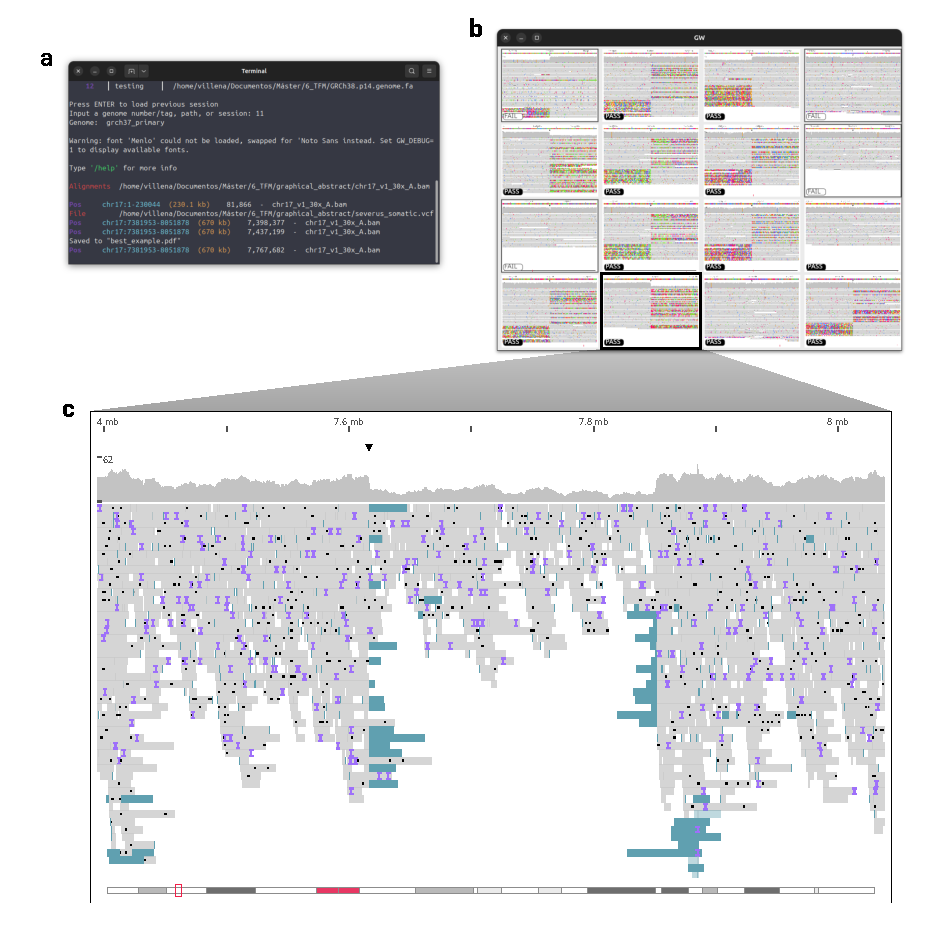
\includegraphics[width=\textwidth]{img/GW_UI.pdf}
    \caption[Alignment-based SV Validation using GW]{Alignment-based SV 
    Validation using GW. The tool is launched through the terminal, initially 
    prompting for reference genome selection (\textbf{a}) and opening an empty graphical
    window. Loading BAM and SV-containing VCF files by dragging them into the 
    graphical window generates a grid of thumbnail images corresponding to 
    VCF-indicated breakpoints (\textbf{b}). Hovering over an image displays breakpoint 
    coordinates in the terminal, while clicking opens a detailed alignment view 
    with chromosome-wide navigation capabilities (\textbf{c}). Users can return to the 
    image grid and toggle True/False buttons in the lower-left corners to track 
    SV validation status, which can be exported as a list for further analysis.}
    \label{fig:GW_UI}
\end{figure}